
%(BEGIN_QUESTION)
% Copyright 2006, Tony R. Kuphaldt, released under the Creative Commons Attribution License (v 1.0)
% This means you may do almost anything with this work of mine, so long as you give me proper credit

Tegn et stigelogikkskjema for en enkel temperaturstyring av en bakeovn med tre temperaturbrytere. Én bryter skal være en høytemperaturalarm som tenner en lampe dersom temperaturen overstiger 450$^{o}$ F. En annen bryter skal styre effekt til varmeelementet, slik at det slås på når temperaturen er under 350$^{o}$ F. Den siste bryteren skal aktivere en "forvarming"-indikatorlampe for å vise kokken at ovnen ennå ikke har nådd driftstemperatur (alle temperaturer under 310$^{o}$ F).

$$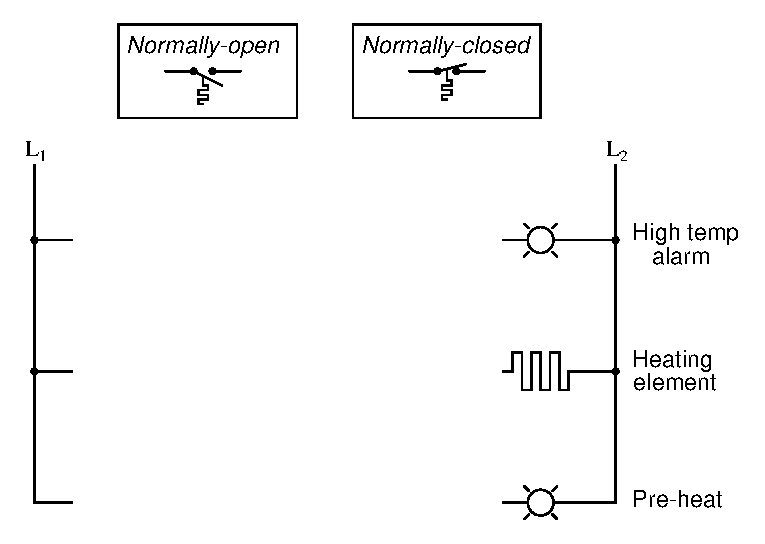
\includegraphics[width=15.5cm]{i00648x01.eps}$$

\vskip 10pt

\noindent
Kreditt gis for korrekt kobling av hver av de tre grein-kretsene. Du {\it må} skrive oppgitt temperaturinnstilling (i grader F) ved hver bryter for å få poeng for den kretsen:

\begin{itemize}
\item{} Høytemperaturalarm-lampe
\item{} Varmeelementstyring
\item{} "Forvarming"-lampe
\end{itemize}

\underbar{file i00648no}
%(END_QUESTION)





%(BEGIN_ANSWER)

$$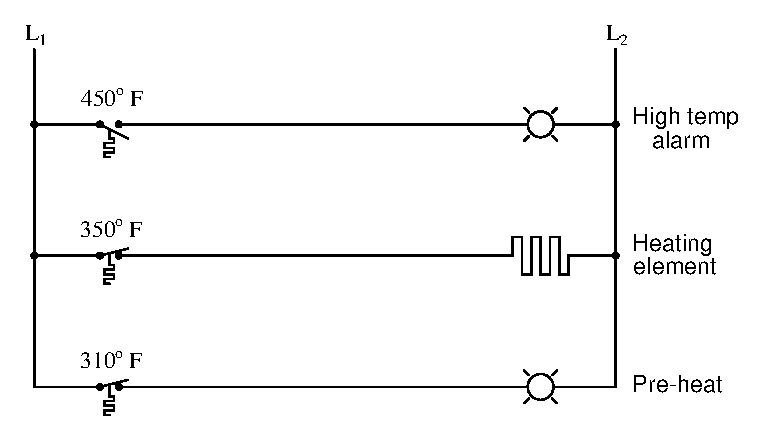
\includegraphics[width=15.5cm]{i00648x02.eps}$$

4 poeng for varmeelementbryteren, 3 poeng for hver av de andre.

%(END_ANSWER)





%(BEGIN_NOTES)

{\bf Denne oppgaven er ment for eksamen, ikke arbeidsark.}

%(END_NOTES)
